\documentclass[12pt,a4paper]{article}
\usepackage[utf8]{inputenc}
\usepackage[T1]{fontenc}
\usepackage{amsmath}
\usepackage{amsfonts}
\usepackage{amssymb}
\usepackage{graphicx}
\usepackage[pdftex]{hyperref} 
\usepackage[left=1cm,right=1cm,top=2cm,bottom=2cm]{geometry}
\author{KONDI Abdoul malik }
\title{Synthèse des projets LARAVEL}
\begin{document}
\maketitle
\tableofcontents
\newpage

\section{Préambule}
Ce document est un résumé du framework PHP LARAVEL (v8). Il est rédigé a partir des travaux
que les équipes de la promotion \textbf{2020} à l'IFNTI (sokodé) on fournis après leurs  stage de fin L2.\\

\newpage
\section{Installation d'un projet laravel via composer}
\subsection{Prérequis}
Pour utiliser le framework LARAVEL il faut avoir:
\begin{itemize}
\item[•] Un PHP v > 7.4.
\item[•] Composer (gestionnaire de dépendance php)[ \href{https://getcomposer.org/download/}{composer link}].
\item[•] Les extensions suivante activé.
\begin{itemize}
\item[-] Version >= 7.2.0,
\item[-] Extension PDO (Le driver pour une connexion avec une base de donnée),
\item[-] Extension \textbf{pgsql} ou \textbf{mysql} ou autre selon votre SGBD.
\item[-] Extension \textbf{mbstring}
\item[-] Extension \textbf{opcache}
\item[-] Extension \textbf{xml}
\item[-] Extension \textbf{curl}
\item[-] Extension \textbf{gd}
\item[-] Extension openSSL
\item[-] Extension json
\item[-] Extension \textbf{fileinfo}
\item[-] Extension \textbf{ctype}
\item[-] Extension \textbf{BCMath}
\item[-] Extension soap
\item[-] Extension zip
\item[-] Extension intl
\item[-] Extension \textbf{common}
\item[-] Extension imagick
\item[-] Extension imap
\end{itemize}
\end{itemize}
Il y a plusieurs façons de créer une application Laravel. La plus classique consiste à utiliser la commande 
\textbf{create-project} de Composer. voici la syntaxe gnérale à utiliser.
\begin{verbatim}
composer create-project laravel/laravel chemain/du/repertoire --prefer-dist "version"
\end{verbatim} 
Créons une application Laravel 8 qui s’appelle \textbf{G\_event}.
\begin{verbatim}
composer create-project laravel/laravel G_event --prefer-dist "8.*"
\end{verbatim}

Une fois l'installation démarré, on a plus qu'a attendre quelques minutes pour que Composer fasse son travail jusqu'au bout. On verra s'afficher une liste de téléchargements. Au final on se retrouve avec cette architechture :

\begin{center}
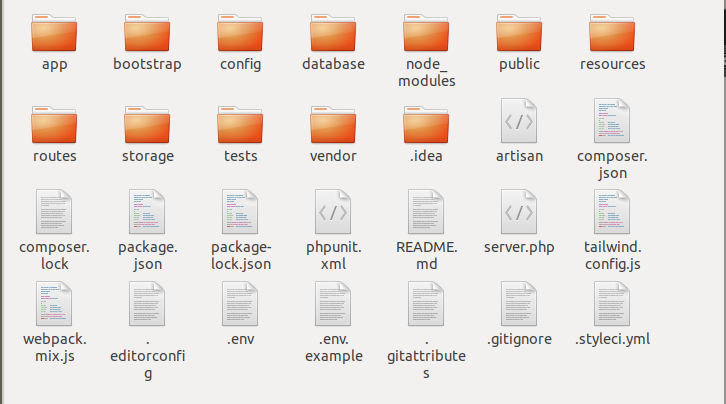
\includegraphics[scale=0.7]{img/groot.png}
\end{center}

Laravel est équiper d'un server pour le developpement qui se lance avec cette commande :
\textbf{php artisan serve}

On peut vérifier que tout fonctionne bien en allant sur l'URL \textit{http://127.0.0.1:8000}. Normalement on doit obtenir cette page.

\begin{center}
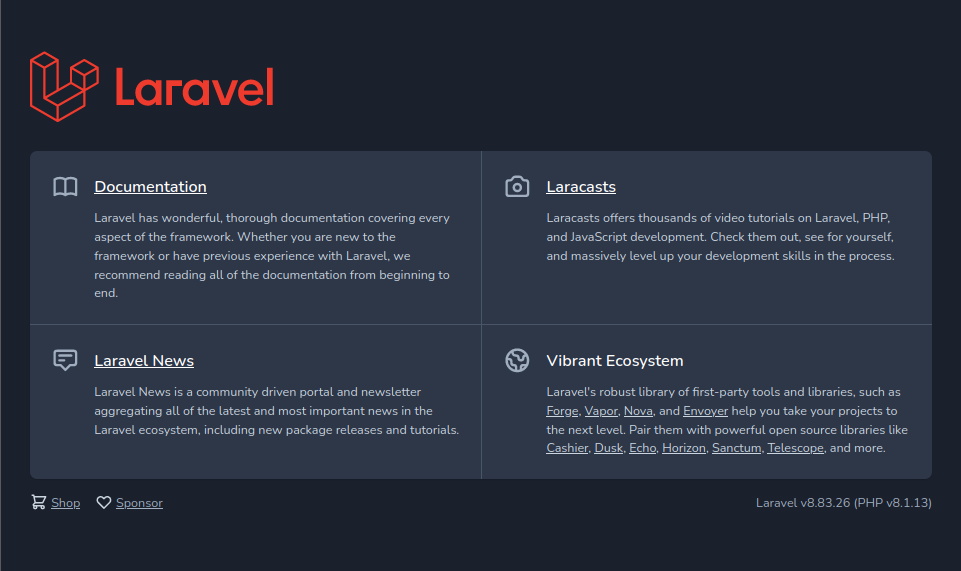
\includegraphics[scale=0.5]{img/laravel_home.png}
\end{center}

Pour des mises à jour ultérieures il suffit encore d'utiliser Composer avec la commande update : \textbf{composer update}

\textbf{Note :} Si vous installez Laravel en téléchargeant directement les fichiers sur Github et en utilisant la commande \textit{composer install}, il vous faut effectuer une action suplémentaires. En effet, dans ce cas la clé de sécurité ne sera pas automatiquement créé et vous allez tomber sur une erreur au lancement. Il faut donc la créer avec la commande.
\textit{php artisan key:generate}.

\subsection{Organisation d'un projet laravel.}
\subsubsection{Répertoire App.}
Le repertoire App est répertoire le plus important de votre projet. C'est lui qui contiendra
votre application, c'est à dire tout votre code php (classes, fonctions ...).

\begin{center}
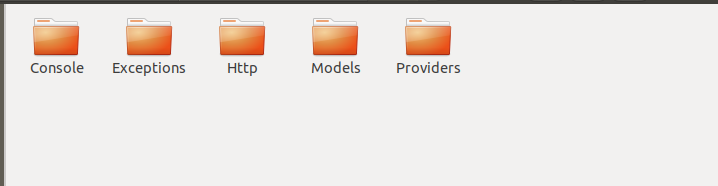
\includegraphics[scale=0.7]{img/gapp.png}
\end{center}

\begin{itemize}
\item[•] Console : toutes les commandes en mode console,
\item[•] Exceptions : pour gérer les erreurs d'exécution,
\item[•] Http : tout ce qui concerne la communication : contrôleurs, middlewares (il y a 8 middlewares
de base qui servent à filtrer les requêtes HTTP) et le kernel,
\item[•] Providers : tous les fournisseurs de services (providers), il y en a déjà 5 au départ. Les providers
servent à initialiser les composants.
\item[•] Models : le dossier des modèles avec déjà un présent qui concerne les utilisateurs.
\end{itemize}

\subsubsection{Autres repertoires.}
Voici une description du contenu des autres dossiers :
\begin{itemize}
\item[•] bootstrap : scripts d'initialisation de Laravel pour le chargement automatique des classes, la fixation de l'environnement et des chemins, et pour le démarrage de l'application,
\item[•] public : tout ce qui doit apparaître dans le dossier public du site : images, CSS, scripts...
\item[•] config : toutes les configurations : application, authentification, cache, base de données, espaces
de noms, emails, systèmes de fichier, session...
\item[•] database : migrations et populations,
Le dossier database permet la gestion de la base données. Il contient trois sous-dossier.
Les migrations sont des fichiers permettant de décrire votre base de données afin de permettre
à Laravel de créer, modifier ou supprimer les tables et les colonnes automatiquement pour vous.
\item[•] resources : vues, fichiers de langage et assets (par exemple les fichiers Sass),
\item[•] routes : la gestion des urls d'entrée de l'application,
\item[•] storage : données temporaires de l'application : vues compilées, caches, clés de session. . .
\item[•] tests : fichiers de tests unitaires,
\item[•] vendor : tous les composants de Laravel et de ses dépendances (créé par composer).
\end{itemize}

\subsubsection{Fichiers de racine.}
Il y a un certain nombre de fichiers dans la racine dont voici les principaux :

\begin{itemize}
\item[•] artisan : outil en ligne (ligne de commande) de Laravel pour des tâches de gestion,
\item[•] composer.json : fichier de référence de composer,
\item[•] package.json : fichier de référence de npm pour les assets,
\item[•] phpunit.xml : fichier de configuration de phpunit (pour les tests unitaires),
\item[•] .env : fichier pour spécifier l'environnement d'exécution.
\end{itemize}
Le fichiers \textbf{.env} contient les mots de passe de vos services ainsi que toutes les
données sensibles de votre application (mot de passe de base de données, adresse de la base de données...). Ce fichier ne doit jamais être partagé. Afin de connaître les informations à
renseigner, il existe un fichier .env.example qui contient uniquement des valeurs d'exemple.
Nous verrons tout cela progressivement dans cette documentation.

\subsubsection{Accessibilité.}
Pour des raisons de securité sur le serveur seul le dossier public est accessible.
Cette configuration n'est pas toujours possible sur un serveur mutualisé (partagé). Il faut alors modifier un tout petit peu Laravel pour que ça fonctionne. Nous en palerons peut être dans la partie déployement.

\newpage
\section{Implémentation du modèle UML.}
Laravel dans sont fonctionnement implémente le pattern MVC (Modèle Vue Controller). Le tableau
explicite mieux cela.
\begin{center}
\begin{tabular}{|c|c|}
\hline 
MVC & LARAVEL \\ 
\hline 
Model & Migration + Model \\ 
\hline 
Vue & Vue \\ 
\hline 
Controlleur & Route + Controller \\ 
\hline 
\end{tabular} 
\end{center}
Voici le modèle UML que nous utiliserons.
\begin{center}
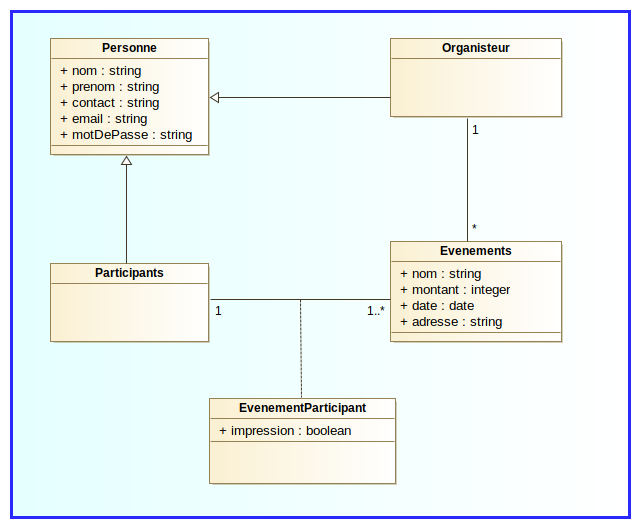
\includegraphics[scale=0.7]{img/model.png}
\end{center} 
\subsection{Les Migrations}
Maintenant que l'application \textbf{G\_event} a été créer nous allons maintement créer une base de données appelé \textbf{gevent}. Une fois que c'est fait nous allons connecter notre application \textbf{LARAVEL} à la base de donnée \textbf{gevent}. Pour le faire rendons nous au niveau du fichier
\textbf{.env}. Vous vous souvenez c'est le fichier dans le quelle on configure l'environement \textbf{LARAVEL} (on peut y spécifier la base de données utilisé, le serveur
de messagerie de notre choix ...). Une fois que le fichier ouvert, modifier les valeurs des
constant \textbf{DB\_CONNECTION}, \textbf{DB\_HOST}, \textbf{DB\_PORT}, \textbf{DB\_DATABASE}, \textbf{DB\_USERNAME}, \textbf{DB\_PASSWORD} comme ceci.

\begin{verbatim}
DB_CONNECTION=pgsql 
DB_HOST=127.0.0.1
DB_PORT=5432
DB_DATABASE=gschool
DB_USERNAME=votre_nom_utilisateur_postgres (Ex : Tamba)
DB_PASSWORD=votre_mot_de_passe_postgres     (EX : 123456789)
\end{verbatim}
Une fois que c'est fait lancer la commande \textbf{php artisant migrate} et relancer la commande \textbf{php artisant serv}.\\
NB : A chaque fois que vous modifier le fichier .env, redémarer toujours le serveur LARAVEL.\\

Maintemant que notre application est connecter à une base de donnée, nous pouvons y créer des migration.
Une migration est un pattern nous permettant de créer des tables dans une base de données tout en étant dans l'application : c' est une représentation en classe PHP des commandes d'un scripte SQL.
Pour créer une migration en LARAVEL on utilise la commande suivante:
\begin{verbatim}
php artisan make:migration create_migration_names_table
\end{verbatim}
NB:
\begin{itemize}
\item[•]  Le nom de la migration doit se terminer par un \textbf{s}. C'est une convention de LARAVEL. Le sens
de cette convention est de dire que nous avons plusieurs objet dans une table. 
\end{itemize}

Maintenant que vous connaissez la commande php qui vous permet de créer des migrations je vous propose de créer les migrations correspondant à notre modèle UML.
C'est fait ? Si non voici ce qu'il fallait faire.
\begin{verbatim}
php artisan make:migration create_organisateurs_table
php artisan make:migration create_evenements_table
php artisan make:migration create_participants_table
php artisan make:migration create_evenements_participants_table
\end{verbatim}

NB:
\begin{itemize}
\item[•] Nous allons utiliser la migration users comme étant la migration du modèle UML personne. Le pourquoi sera expliqué par la suite.
\item[•] Lorsque nous avons une relation *-* entre deux modèles sera est implémenté en LARAVEL par une migration intermédiaire (comme en \textbf{SQL}). Le nom de cette dernière est composé des noms des deux modèles avec un \textbf{s} à la fin de 
chacune d'elle. Encore une fois c'est la convention qui l'oblige.
\end{itemize}

Une fois que les migration crée voici leur contenue.
\begin{itemize}
\item[•] users
\begin{verbatim}
<?php

use Illuminate\Database\Migrations\Migration;
use Illuminate\Database\Schema\Blueprint;
use Illuminate\Support\Facades\Schema;

return new class extends Migration
{
    /**
     * Run the migrations.
     *
     * @return void
     */
    public function up()
    {
        Schema::create('users', function (Blueprint $table) {
            $table->bigIncrements('id_user');
            $table->string('nom');
            $table->string('prenom');
            $table->string('contact');
            $table->string('email')->unique();
            $table->timestamp('email_verified_at')->nullable();
            $table->string('password');
            $table->rememberToken();
            $table->timestamps();
        });
    }

    /**
     * Reverse the migrations.
     *
     * @return void
     */
    public function down()
    {
        Schema::dropIfExists('users');
    }
};

\end{verbatim}
\item[•] organisateur
\begin{verbatim}
<?php

use Illuminate\Database\Migrations\Migration;
use Illuminate\Database\Schema\Blueprint;
use Illuminate\Support\Facades\Schema;

class CreateOrganisateursTable extends Migration
{
    /**
     * Run the migrations.
     *
     * @return void
     */
    public function up()
    {
        Schema::create('organisateurs', function (Blueprint $table) {
            $table->bigIncrements('id_organisateur');
            $table->bigInteger("personne");
            $table->timestamps();
            $table->foreign("personne")->references("id_user")->on("users");

        });
    }

    /**
     * Reverse the migrations.
     *
     * @return void
     */
    public function down()
    {
        Schema::dropIfExists('organisateurs');
    }
}

\end{verbatim}
\item[•] evenements
\begin{verbatim}
<?php

use Illuminate\Database\Migrations\Migration;
use Illuminate\Database\Schema\Blueprint;
use Illuminate\Support\Facades\Schema;

return new class extends Migration
{
    /**
     * Run the migrations.
     *
     * @return void
     */
    public function up()
    {
        Schema::create('evenements', function (Blueprint $table) {
            $table->bigIncrements("id_evenement");
            $table->string('nom');
            $table->float('montant');
            $table->date('date'); // date et heur
            $table->json('adresse');
            $table->bigInteger('organisateur');
            $table->timestamps();
            $table->foreign("organisateur")->references("id_user")->on("users");
        });
    }

    /**
     * Reverse the migrations.
     *
     * @return void
     */
    public function down()
    {
        Schema::dropIfExists('evenements');
    }
};

\end{verbatim}
\item[•] participants
\begin{verbatim}
<?php

use Illuminate\Database\Migrations\Migration;
use Illuminate\Database\Schema\Blueprint;
use Illuminate\Support\Facades\Schema;

return new class extends Migration
{
    /**
     * Run the migrations.
     *
     * @return void
     */
    public function up()
    {
        Schema::create('participants', function (Blueprint $table) {
            $table->bigIncrements('id_participant');
            $table->bigInteger("personne");
            $table->timestamps();
            $table->foreign("personne")->references("id_user")->on("user");
        });
    }

    /**
     * Reverse the migrations.
     *
     * @return void
     */
    public function down()
    {
        Schema::dropIfExists('participants');
    }
};


\end{verbatim}
\item[•] evenements\_participants
\begin{verbatim}
<?php

use Illuminate\Database\Migrations\Migration;
use Illuminate\Database\Schema\Blueprint;
use Illuminate\Support\Facades\Schema;

return new class extends Migration
{
    /**
     * Run the migrations.
     *
     * @return void
     */
    public function up()
    {
        Schema::create('evenements_participants', function (Blueprint $table) {
            $table->foreignId("id_evenement");
            $table->foreignId("id_participant");
            $table->enum("impression", array(0,1));
            $table->timestamps();
        });
    }

    /**
     * Reverse the migrations.
     *
     * @return void
     */
    public function down()
    {
        Schema::dropIfExists('evenements_participants');
    }
};

\end{verbatim}
\end{itemize}

Nous pouvez constater qu'une migration est une class \textbf{PHP} qui hérite de la class
\textbf{Migration} et qu'elle contient deux méthodes : \textbf{up et down}.

\begin{itemize}
\item[•] \textbf{up} est la méthode dans la quelle nous allons indiquer ce qui se passe lorsqu'on lance la migation.
\item[•] \textbf{down} est la méthode dans la quelle nous indiquons le directive à exécuter lorque la migration
est anuller.
\end{itemize}

\subsubsection{documents de référence}
\begin{itemize}
\item[•] https://laravel.com/docs/8.x/migrations
\item[•] https://laravel.com/docs/8.x/seeding
\end{itemize}

\subsection{Les Models}
Un modèle en LARAVEL implémente l'ORM (Object-Relational Mapper). L'ORM permet à un modèle de 
communiquer directement avec la base de donnée.\\

Pour créer un model en LARAVEL on utilise la commande suivante:
\begin{verbatim}
php artisan make:model NomModel
\end{verbatim}
NB: Il n'y a pas de \textbf{s} à la fin du nom d'un modèle et le nom d'un modèle doit commencer par 
une lettre majuscule.

Maintenant que vous connaissez la commande php LARAVEL qui vous permet de créer un modèle je vous
propose de créer les modèles correspondant à nos migrations.
C'est fait ? Si non voici ce qu'il fallait faire.
\begin{verbatim}
php artisan make:model Organisateur
php artisan make:model Evenement
php artisan make:model Participant
\end{verbatim}

Le modèle User existe déjà c'est pour cela nous l'avons pas créer.
Vous vous demandez sûrement pourquoi nous n'avons pas créer de modèle pour la migration association ?
La réponse à cette que la méthode que nous allons utiliser ici au niveau du modèle pour régler ce
problème ne nécessite pas de modèle association.

Voici le contenue de nos modèles.\\

\begin{itemize}
\item[•] User
\begin{verbatim}
<?php

namespace App\Models;

// use Illuminate\Contracts\Auth\MustVerifyEmail;
use Illuminate\Database\Eloquent\Factories\HasFactory;
use Illuminate\Foundation\Auth\User as Authenticatable;
use Illuminate\Notifications\Notifiable;
use Laravel\Sanctum\HasApiTokens;

class User extends Authenticatable
{
    use HasApiTokens, HasFactory, Notifiable;

    /**
     * The attributes that are mass assignable.
     *
     * @var array<int, string>
     */
    protected $fillable = [
        'nom',
        'prenom',
        'contact',
        'email',
        'password',
    ];

    protected $primaryKey = 'id_user';

    /**
     * The attributes that should be hidden for serialization.
     *
     * @var array<int, string>
     */
    protected $hidden = [
        'password',
        'remember_token',
    ];

    /**
     * The attributes that should be cast.
     *
     * @var array<string, string>
     */
    protected $casts = [
        'email_verified_at' => 'datetime',
    ];

    public function organisateur()
    {
        return $this->hasOne(Organisateur::class,"personne");
    }

    public function participant()
    {
        return $this->hasOne(Participant::class,"personne");
    }
}

\end{verbatim}
\item[•] Organisateur
\begin{verbatim}
<?php

namespace App\Models;

use Illuminate\Database\Eloquent\Factories\HasFactory;
use Illuminate\Database\Eloquent\Model;

class Organisateur extends Model
{
    use HasFactory;
    protected $fillable = ['personne'];
    protected $primaryKey = 'id_organisateur';

    public function user()
    {
        return $this->belongsTo(User::class,"personne");
    }

    public function evenements()
    {
        return $this->hasMany(Evenement::class, "organisateur");
    }
}
\end{verbatim}
\item[•] Participant
\begin{verbatim}
<?php

namespace App\Models;

use Illuminate\Database\Eloquent\Factories\HasFactory;
use Illuminate\Database\Eloquent\Model;

class Participant extends Model
{
    use HasFactory;
    protected $fillable = ['personne'];
    protected $primaryKey = 'id_participant';

    public function user()
    {
        return $this->belongsTo(User::class,"personne");
    }

    public function evenements(){
        return $this->belongsToMany(Evenement::class, "evenements_participants", 
        "id_evenement", "id_participant")
                    ->withPivot(array("impression"));
    }
}
\end{verbatim}
\item[•] Evenement
\begin{verbatim}
<?php

namespace App\Models;

use Illuminate\Database\Eloquent\Factories\HasFactory;
use Illuminate\Database\Eloquent\Model;

class Evenement extends Model
{
    use HasFactory;

    protected $fillable = [
        'nom',
        'montant',
        'organisateur',
        'date',
        'adresse',
    ];

    protected $casts = [
        'adresse' => 'array'
    ];

    protected $dates = [
        'date',
    ];

    protected $primaryKey = 'id_evenement';

    public function organisateur()
    {
        return $this->belongsTo(Organisateur::class, "organisateur");
    }

    public function participants(){
        return $this->belongsToMany(Participant::class, "evenements_participants", 
        "id_evenement", "id_participant")
                    ->withPivot(array("impression"));
    }
}

\end{verbatim}
\end{itemize}

Explication :\\
\begin{itemize}
\item[•] La variable \$fillable permet d'indiquer les colonnes à accepter lors de la création
de l'objet.
\item[•] La variable \$primaryKey permet d'indiquer la clé primaire de la relation.
\item[•] La relation  1 - 1 est implémenter avec \textbf{hasOne} et \textbf{belongTo}
\item[•] La relation  1 - * est implémenter avec \textbf{hasMany} et \textbf{belongTo}
\item[•] La relation  * - * est implémenter avec \textbf{belongToMany} et \textbf{belongToMany}
\end{itemize}
\subsubsection{documents de référence}
\begin{itemize}
\item https://laravel.com/docs/8.x/eloquent
\item https://laravel.com/docs/8.x/eloquent-relationships
\end{itemize}


\subsection{Les Controllers}
Un contrôleur est une classe PHP qui permet de relier plusieurs vues à un modèle. On peut énumérer
sept (7) méthodes se trouvant dans un contrôleur à savoir : \\
\textit{index}, \textit{create}, \textit{store}, \textit{show}, \textit{edite}, \textit{update}, \textit{delete}.\par
Utilisation et utilité de chaque méthodes.\\

\begin{center}
\begin{tabular}{|c|c|c|c|c|c|}
\hline 
Verb & URI & Action & Route Name & Signification \\ 
\hline 
GET & /photos & index & photos.index & Affiche la liste des objets Photo \\ 
\hline 
GET & /photos/create & create & photos.create & Affiche un formulaire d'enregistrement \\ 
\hline 
POST & /photos & store & photos.store & enregistrement d'un objet Photo\\ 
\hline 
GET & /photos/{photo} & show & photos.show & Affiche les détails d'un objet Photo \\ 
\hline 
GET & /photos/{photo}/edit & edit & photos.edit & Affiche un formulaire d'édition \\ 
\hline 
PUT/PATCH & /photos/{photo} & update & photos.update & Met à jour un objet Photo \\ 
\hline 
DELETE & /photos/{photo} & destroy & photos.destroy & Supprime un objet Photo \\ 
\hline 
\end{tabular} 
\end{center}

Pour créer un contrôleur on utilise la commande suivante:
\begin{verbatim}
php artisan make:controller NomController
\end{verbatim}

Je vous laisse donc créer les contrôleurs correspondant à nos modèle. C'est fais ?
si telle n'est pas le cas voici ce qu'il fallait faire.

\begin{itemize}
\item[•] EvenementController
\begin{verbatim}
php artisan make:controller EvenementController
\end{verbatim}
\item[•] participantController
\begin{verbatim}
php artisan make:controller participantController
\end{verbatim}
\end{itemize}

Maintenant comment accéder à ces méthodes via le navigateur ? Pour le faire il vas falloir comprendre 
la notion de route.

\subsubsection{Documents de référence}
\begin{itemize}
\item https://laravel.com/docs/8.x/controllers
\end{itemize}

\subsection{Les Routes}
Une route est le moyen par le quel un contrôleur peut communiquer avec une vue.\\
Pour créer une route on se rend dans le fichier \textbf{route/web.php} et on n'y ajoute une ligne sous
la forme suivante.
\begin{verbatim}
route:methodeHttp(uri, méthodeController)->name(nom);
\end{verbatim}

Explication :
\begin{itemize}
\item[•] \textbf{uri} est un suffixe qui sera ajouté à l'url de base (\textit{http://127.0.0.1/uri}) pour former une nouvelle url menant à la méthode indiqué dans la route.
\item[•] La \textbf{methodeHttp} est la moyen par le quelle nous accédons à la méthode (get, post, put ...).
\item[•] Avec le nom de la route nous pouvons l'utiliser n'importe où dans un fichier \textbf{php}. 
\end{itemize}

Exemple de route : 
\begin{verbatim}
Route::get('/', function () {
    return "Hello";
});

Route::get('/', function () {
    return view('welcome');
});

Route::post('enregistrement_abonne', 
'App\Http\Controllers\AbonneController@store')->name('storeAbonne');

Route::get('lire_pdf/{ouvragesElectronique}/lecture',
 [LivreNumeriqueController::class, 'readPdf'])->name('lirePDF');

Route::put('mise_a_jour_des_abonnes/{abonne}', 'App\Http\Controllers\
AbonneController@update')->name('updateAbonne');
 
\end{verbatim}

Maintenant que vous savez comment créer des routes créer des routes pour nos contrôleur. C'est fais ?
voici ce qu'il fallait faire.

\begin{verbatim}
// routes evenements
Route::get('liste_des_evenements', [\App\Http\Controllers\EvenementController::class, 
'index'])->name('listeEvenements');
Route::get('formulaire_enregistrement_evenement', [\App\Http\Controllers\EvenementController
::class, 'create'])->name('formulaireEnregistrementEvenement');
Route::post('enregistrement_evenement', [\App\Http\Controllers\EvenementController::class, 
'store'])->name('enregistrementEvenement');
Route::get('afficher_evenement/{evenement}', [\App\Http\Controllers\EvenementController
::class, 'destroy'])->name('afficherEvenement');
Route::get('formulaire_editer_evenement/{evenement}/editer', [\App\Http\Controllers
\EvenementController::class, 'edit'])->name('formulaireEditerEvenement');
Route::put('mise_a_jour_evenement/{evenement}', [\App\Http\Controllers\EvenementController
::class, 'update'])->name('miseAjourEvenement');
Route::delete('supprimer_evenement/{evenement}', [\App\Http\Controllers\EvenementController
::class, 'destroy'])->name('supprimerEvenement');
Route::put('mise_a_jour_evenement/{evenement}', [\App\Http\Controllers\EvenementController
::class, 'update'])->name('miseAjourEvenement');

// routes participants
Route::get('liste_des_participants', [\App\Http\Controllers\EvenementController::class, 
'index'])->name('listeparticipants');
Route::get('formulaire_enregistrement_participant', [\App\Http\Controllers\
EvenementController::class, 'create'])->name('formulaireEnregistrementparticipant');
Route::post('enregistrement_participant', [\App\Http\Controllers\EvenementController
::class, 'store'])->name('enregistrementparticipant');
Route::get('afficher_participant/{participant}', [\App\Http\Controllers\
EvenementController::class, 'destroy'])->name('afficherparticipant');
Route::get('editer_participant/{participant}/editer', [\App\Http\Controllers
\EvenementController::class, 'edit'])->name('editerparticipant');
Route::put('mise_a_jour_participant/{participant}', [\App\Http\Controllers\
EvenementController::class, 'update'])->name('miseAjourparticipant');
Route::delete('supprimer_participant/{participant}', [\App\Http\Controllers\
EvenementController::class, 'destroy'])->name('supprimerparticipant');

\end{verbatim}

\subsubsection{Documents de référence}
\begin{itemize}
\item https://laravel.com/docs/8.x/routing
\end{itemize}

\subsection{Les vues}
Sous Laravel, pour afficher correctement une page Web dans le navigateur, il faut utiliser une vue. C'est la vue qui est en charge de générer le code HTML. Elle utilisera pour cela, en plus des balises HTML, des directives et instructions que le moteur d'affichage Blade met à sa disposition.\\
Blade est un langage de template comme jindja2. 
Essayons d'afficher la liste des événements. Pour le faire je vous pousse à aller dans la documentation
de laravel partie \textbf{Blade Templates} pour pouvoir réalisé cette page.
C'est fait ?\\

voici ce qu'il fallait faire.

\begin{verbatim}
<html>
    <head>
        <meta charset="utf-8">
        <title>Liste</title>
    </head>
    <body>
        <div>
            <form method="get" action="{{route('formulaireEnregistrementEvenement')}}">
                <input type="submit" name="ajouter" value="Ajouter">
            </form>
            <form method="get" action="{{route('formulaireImportExcel')}}">
                <input type="submit" name="ajouter" value="Importer">
            </form>
        </div>
        @if($evenements && $evenements->count() > 0)
            <h1>{{ Liste des événements }}</h1>
            <table border="1">
                <thead>
                <th>Nom</th>
                <th>Montant</th>
                <th>Date</th>
                <th>Adresse</th>
                <th>Organisation</th>
                <th>Nombre de participant</th>
                <th>Participer</th>
                <th>Editer</th>
                <th>Supprimer</th>
                </thead>
                <tbody>
                @foreach($evenements as $event)
                    <tr>
                        <td>{{ $event->nom }}</td>
                        <td>{{ $event->montant }}</td>
                        <td>{{ $event->date }}</td>
                        <td>{{ $event->adresse['ville'] }}</td>
                        <td>{{ $event->organisateur }}</td>
                        <td></td>
                        <td>
                            <form method="" action="">
                                @csrf
                                <input type="submit" value="Participer">
                            </form>
                        </td>
                        <td>
                            <form method="" action="">
                                @csrf
                                <input type="submit" value="Editer">
                            </form>
                        </td>
                        <td>
                            <form method="" action="">
                                @csrf
                                @method('delete')
                                <input type="submit" value="Supprimer">
                            </form>
                        </td>
                    </tr>
                @endforeach
                </tbody>
            </table>
        @else
            <h1>Aucun événement enregister.</h1>
        @endif

    </body>
</html>

\end{verbatim}

Maintenant que c'est fait nous allons passer à la réalisation de toute nos vues. Pour cela nous allons
créer deux répertoire dans le dossier ressource/vue qui se nomme respectivement événements et participants.\\
Dans chaque répertoire nous allons créer quatre fichiers (index, create, edite, show) avec l’extension \textbf{.blade.php}. Comme l'indique la figure suivante.

Nous allons éditer ensemble les fichiers du dossier événements. Je vous laisse faire tous seul l'édition
des fichier du répertoire participant.

\begin{itemize}
\item[•] \textbf{create.blade.php} :
\begin{verbatim}
<html>
<head>
    <meta charset="utf-8">
    <title>Liste</title>
</head>
<body>
    <main>
        <h1>Formulaire d'enregistrement d'un événements.</h1>
        <form method="post" action="{{ route('enregistrementEvenement') }}">
            @csrf
            <div>
                <label>Nom</label>
                <input type="text" name="nom">
            </div>
            <div>
                <label>Montant</label>
                <input type="number" name="montant">
            </div>
            <div>
                <label>Date</label>
                <input type="datetime-local" name="date">
            </div>
            <div>
                <label>Adresse</label>
                <table>
                    <thead>
                        <th>Ville</th>
                        <th>Quartier</th>
                        <th>lieu</th>
                    </thead>
                    <tbody>
                        <tr>
                            <td>
                                <input type="text" name="ville">
                            </td>
                            <td>
                                <input type="text" name="quartier">
                            </td>
                            <td>
                                <input type="text" name="lieu">
                            </td>
                        </tr>
                    </tbody>
                </table>
            </div>
            <div>
                <label>Organisateur</label>
                <select name="organisateur">
                    <option value="">Sélectionner</option>
                    @foreach($organisateurs as $organisateur)
                        <option value="{{ $organisateur->user->id_user }}">
                        {{ $organisateur->user->nom }}</option>
                    @endforeach
                </select>
            </div>
            <input type="submit" value="enregister">
        </form>
    </main>
</body>
</html>

\end{verbatim}
\item[•] \textbf{edite.blade.php} :
\begin{verbatim}
<html>
<head>
    <meta charset="utf-8">
    <title>Liste</title>
</head>
<body>
<main>
    <h1>Edition de l' événements {{ $evenement->id_evenement }}.</h1>
    <form method="post" action="{{ route('miseAjourEvenement', $evenement) }}">
        @csrf
        @method('put')
        <div>
            <label>Nom</label>
            <input type="text" name="nom" 
            value="{{ $evenement->nom }}">
        </div>
        <div>
            <label>Montant</label>
            <input type="number" name="montant" 
            value="{{ $evenement->montant }}">
        </div>
        <div>
            <label>Date</label>
            <input type="datetime-local" name="date" 
            value="{{ $evenement->date }}">
        </div>
        <div>
            <label>Adresse</label>
            <table>
                <thead>
                <th>Ville</th>
                <th>Quartier</th>
                <th>lieu</th>
                </thead>
                <tbody>
                <tr>
                    <td>
                        <input type="text" name="ville" 
                        value="{{ $evenement->adresse["ville"] }}">
                    </td>
                    <td>
                        <input type="text" name="quartier" 
                        value="{{ $evenement->adresse["quartier"] }}">
                    </td>
                    <td>
                        <input type="text" name="lieu" 
                        value="{{ $evenement->adresse["lieu"] }}">
                    </td>
                </tr>
                </tbody>
            </table>
        </div>
        <div>
            <label>Organisateur</label>
            <select name="organisateur">
                <option value="">Sélectionner</option>
                @foreach($organisateurs as $organisateur)
                    <option value="{{ $organisateur->user->id_user }}" 
                    {{ $evenement->organisateur == $organisateur->user->id_user ? 
                    "selected" : "" }}>{{ $organisateur->user->nom }}</option>
                @endforeach
            </select>
        </div>
        <input type="submit" value="Mettre à jour">
    </form>
</main>
</body>
</html>
\end{verbatim}
\end{itemize} 
C'est bien beau tous ça mais ça ne marchera pas. Pourquoi ? car nous avons pas encore définit le corps
des méthodes du contrôleur \textbf{EvenementController}.\\
Remplissez les comme ceci. Pour plus d'information allez voir la documentation (partie contrôler).
\begin{verbatim}
 public function index()
    {
        return view('evenement.index')->with(['evenements' => Evenement::all(),]);
    }
 public function create()
    {
        $organisateurs = Organisateur::all();
        return view('evenement.create', compact('organisateurs'));
    }
  public function store(Request $request)
    {
        $request->validate([
            'nom' => 'required',
            'montant' => 'required',
            'date' => 'required',
            'ville' => 'required',
            'quartier' => 'required',
            'lieu' => 'required',
            'organisateur' => 'required',
        ]);

        $request->adresse = array(
            'ville' => $request->ville,
            'quartier' => $request->quartier,
            'lieu' => $request->lieu,
        );

        $request->datetime = explode("T", $request->date);
        $request->date = $request->datetime[0];
        $request->time = $request->datetime[1];

        Evenement::create([
            'nom' => $request->nom,
            'montant' => $request->montant,
            'date'=> Carbon::createFromFormat("Y-m-d H:i", 
            $request->date." ".$request->time),
            'adresse' => $request->adresse,
            'organisateur' => User::all()->where('id_user', '=',
             $request->organisateur)->first()->id_user,
        ]);

public function edit(Evenement $evenement)
    {
        $organisateurs = Organisateur::all();
        return view('evenement.edite', 
        compact(['evenement', 'organisateurs']));
    }

public function update(Request $request, Evenement $evenement)
    {
        $request->validate([
            'nom' => 'required',
            'montant' => 'required',
            'date' => 'required',
            'ville' => 'required',
            'quartier' => 'required',
            'lieu' => 'required',
            'organisateur' => 'required',
        ]);

        $request->adresse = array(
            'ville' => $request->ville,
            'quartier' => $request->quartier,
            'lieu' => $request->lieu,
        );
        $request->datetime = explode("T", $request->date);
        $request->date = $request->datetime[0];
        $request->time = $request->datetime[1];

        //dd(Carbon::createFromFormat("Y-m-d H:i", 
        $request->date." ".$request->time));

        $evenement->nom = $request->nom;
        $evenement->montant = $request->montant;
        $evenement->adresse = $request->adresse;
        $evenement->date = Carbon::createFromFormat("Y-m-d H:i", 
        $request->date." ".$request->time);
        $evenement->organisateur = $request->organisateur;
        $evenement->save();

        return redirect()->route('listeEvenements');
    }
    
public function destroy(Evenement $evenement)
    {
        $participants = $evenement->participants;
        foreach ($participants as $participant){
            $evenement->participants()
            ->detach($participant->id_participant);
        }
        $evenement->delete();
        return redirect()->route('listeEvenements');
    }
\end{verbatim}

\subsubsection{Documents de référence}
\begin{itemize}
\item https://laravel.com/docs/8.x/validation
\item https://laravel.com/docs/8.x/views
\end{itemize}

Image récapitulatif:
\begin{center}
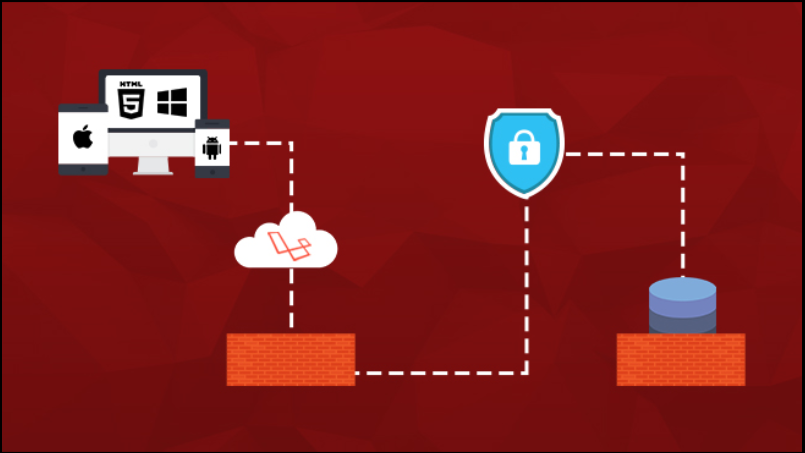
\includegraphics[scale=0.5]{img/laravel.png}
\end{center}
\begin{center}
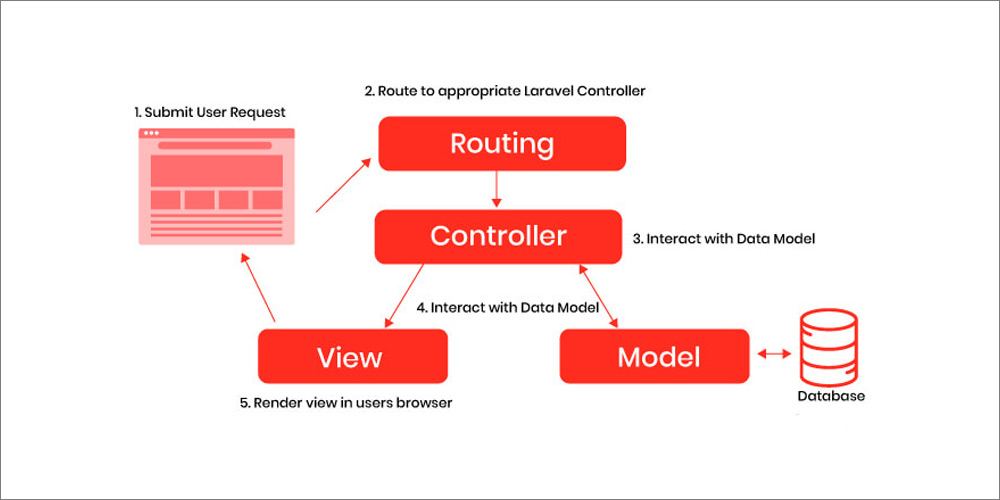
\includegraphics[scale=0.5]{img/MVC-Support.jpg}
\end{center}

\section{Les Services Providers}

\subsection{Helpers}
Les helpers sont des méthodes static permettant d'aider les vues. Il sont accessible n'importe où dans
l'application laravel.
Vous pouvez remarquer que jusqu’à  présent l'adresse de l'événement n'es pas précis.
Nous souhaitons afficher l'adresse sous cette forme : \textit{"À "+ville+", "+quartier+" vers le "+lieu}. Comment faire ? C'est justement le rôle d'un helper.
Pour pouvoir utiliser les helpers dans un projet laravel il va vous falloir installer le module package 
helper. La commande suivante permet de faire.
\begin{verbatim}
composer require mercuryseries/laravel-helpers
\end{verbatim}
Une fois que c'est fait nous allons créer le répertoire \textbf{Helpers} dans le répertoire
\textbf{app/}. C'est fait ? Okay. Nous allons créer la classe \textbf{EvenementHelper} dans le répertoire précédemment crée.  Cette classe aura pour méthode static \textbf{afficherAdresse}.
Je vous laisse essayer de remplir ce fichier avant de continuer. C'est fait ? Voici ce qu'il faut faire.

\begin{verbatim}
<?php

namespace App\Helpers;

class EvenementHelper
{
    
    public static function afficherAdresse(array $array)
    {
        return "À ".$array['ville'].", ".$array['quartier']." vers le ".$array['lieu'];
    }
}
\end{verbatim}

Comment l'utiliser dans nos vues ?\\
Pour l'utiliser au niveau des vues (dans notre cas dans la vue evenement/index) on import l'helper comme
ceci.
\begin{verbatim}
<td>{{ \App\Helpers\EvenementHelper::afficherAdresse($event->adresse) }}</td>
\end{verbatim}

Avant l'helper :
\begin{center}
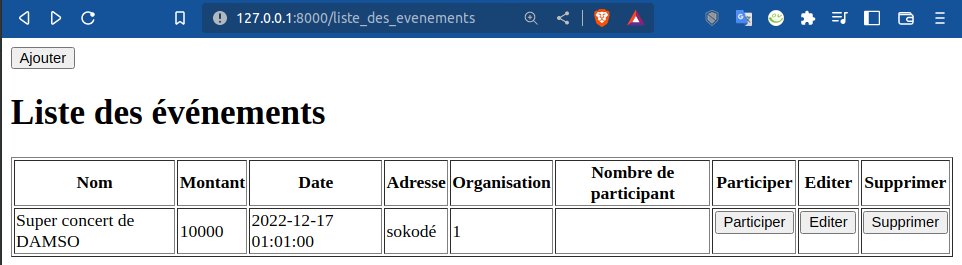
\includegraphics[scale=0.5]{img/evenement_before_helper.png}
\end{center}
Après l'helper :
\begin{center}
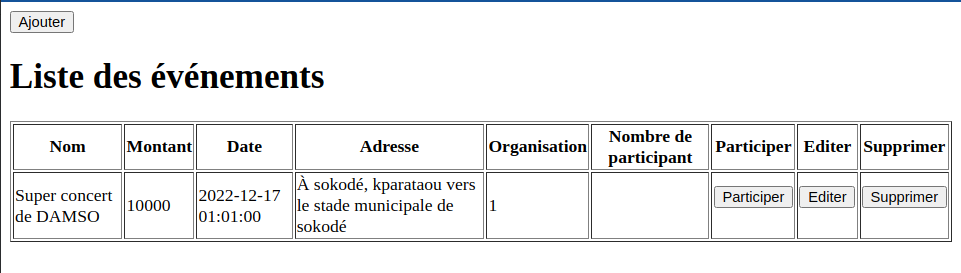
\includegraphics[scale=0.5]{img/evenement_after_helper.png}
\end{center}

\subsection{Service}

Les services sont comme les helpers mais eux ils sont axé côté modèle.
Vous pouvez remarquer que pour valider les formulaires aux niveau des méthodes \textbf{store et update}
du contrôleur \textbf{evenementController} on écrit les mêmes instructions. Et vous le savez bien dupliquer du code c'est mal. Les services sont la en partie pour nous aider à régler cela.
Pour utiliser un service il n'y a pas de module à installer. on crée seulement le répertoire \textbf{Service} dans \textbf{app/}. Une fois le répertoire créer, on créer une classe service et on
n'y définit le plus souvent des méthodes static. Nous allons donc créer un classe php qui s'appelle
\textbf{EvenementService} dans la quelle nous allons créer la méthodes static \textbf{} qui prend la variable \$request en parametre comme ceci.

\begin{verbatim}
<?php

namespace App\Service;

use Illuminate\Http\Request;

class EvenementService
{
    public static function validateFromRequest(Request $request)
    {
        $request->validate([
            'nom' => 'required',
            'montant' => 'required',
            'date' => 'required',
            'ville' => 'required',
            'quartier' => 'required',
            'lieu' => 'required',
            'organisateur' => 'required',
        ]);
    }
}
\end{verbatim}

Comment l'utiliser dans nos contrôleurs ?\\
Pour l'utiliser au niveau des contrôleurs (dans notre cas dans le contrôleur evenementController) on utilise le service comme
ceci.
\begin{verbatim}
public function store(Request $request)
    {
        EvenementService::validateFromRequest($request);

        $request->adresse = array(
            'ville' => $request->ville,
            'quartier' => $request->quartier,
            'lieu' => $request->lieu,
        );

        $request->datetime = explode("T", $request->date);
        $request->date = $request->datetime[0];
        $request->time = $request->datetime[1];

        Evenement::create([
            'nom' => $request->nom,
            'montant' => $request->montant,
            'date'=> Carbon::createFromFormat("Y-m-d H:i", $request->date." ".$request->time),
            'adresse' => $request->adresse,
            'organisateur' => User::all()->where('id_user', '=', $request->organisateur)->first()->id_user,
        ]);

        return redirect()->route('listeEvenements');
    }

......... 
.........
.........    
    
    public function update(Request $request, Evenement $evenement)
    {
        EvenementService::validateFromRequest($request);

        $request->adresse = array(
            'ville' => $request->ville,
            'quartier' => $request->quartier,
            'lieu' => $request->lieu,
        );
        $request->datetime = explode("T", $request->date);
        $request->date = $request->datetime[0];
        $request->time = $request->datetime[1];

        //dd(Carbon::createFromFormat("Y-m-d H:i", $request->date." ".$request->time));

        $evenement->nom = $request->nom;
        $evenement->montant = $request->montant;
        $evenement->adresse = $request->adresse;
        $evenement->date = Carbon::createFromFormat("Y-m-d H:i", $request->date." ".$request->time);
        $evenement->organisateur = $request->organisateur;
        $evenement->save();

        return redirect()->route('listeEvenements');
    }
\end{verbatim}

\subsection{Authentification avec breez}
Il existe deux systèmes d'authentification avec LARAVEL à savoir \textbf{UI} et \textbf{BREEZ}. Mais dans ce document nous allons voir \textbf{BREEZ}. Pour installer
breez dans laravel voici comment s'y prendre.\\
Lancer les commandes suivante mais avant sauvegarder vos routes autre par que dans 
l'application LARAVEL car Breez les supprimera.

\begin{verbatim}
composer require laravel/breeze:1.9.2
php artisan breeze:install
 
npm install
npm run dev
php artisan migrate
\end{verbatim}

Une fois breez installer, reporter vos route dans le fichier web.php.
Si vous voulez qu'un utilisateur soi authentifier avant d'accéder au tableau de bord
voici ce qu'il faut faire.
\begin{verbatim}
Route::group(['middleware' => ['auth']], function () {
    Route::get('/dashboard', function () {
        return view('dashboard');
    })->name('dashboard');
});
\end{verbatim}

Preuve:

Maintenant vous allez vous demander sûrement comment gérer les rôles et les permissions ?
Ne vous inquiétez pas. Pour gérer les rôles et le permissions nous allons utiliser
LARAVEL spatie. Pour l'installer lancer la commande suivante.

\begin{verbatim}
 composer require spatie/laravel-permission
\end{verbatim}

Après l'installation ajouter dans le fichier config/app.php la ligne suivante :
\begin{verbatim}
Spatie\Permission\PermissionServiceProvider::class,
\end{verbatim}

Maintenant il faut publier le service provider comme ceci:
\begin{verbatim}
php artisan vendor:publish --provider="Spatie\Permission\PermissionServiceProvider"
\end{verbatim}

Enfin nettoyez le cache et lancer a nouveau les migrations.
\begin{verbatim}
php artisan config:clear
php artisan migrate
\end{verbatim}

A cette étape on peut commencer à utiliser spatie mais nous allons ajouter trois ligne 
dans la variable \textit{routeMiddleware} comme ceci.
\begin{verbatim}
protected $routeMiddleware = [
        .............................
        .............................
        .............................
        'role' => \Spatie\Permission\Middlewares\RoleMiddleware::class,
        'permission' => \Spatie\Permission\Middlewares\PermissionMiddleware::class,
        'role_or_permission' => \Spatie\Permission\Middlewares\RoleOrPermissionMiddleware::class,
    ];
\end{verbatim}

Cela nous permettra d'avoir accès aux variable \textbf{role, permission et role\_or\_permission} dans le fichier \textbf{web.php}.

Testons maintenant spatie. Nous allons créer:
\begin{itemize}
\item[•]  Deux rôles : public et organisateur.
\item[•]  Deux Utilisateurs : l'un ayant le rôle public et l'autre organisateur.
\item[•]  L'organisateur pourra voir le nombre de participant et mais le public non.
\item[•] De plus l'organisateur pourra supprimer un événement mais le public non.
\end{itemize}

\begin{itemize}
\item[•] Création de deux rôles :

\end{itemize}

\subsubsection{Documents de référence}
\begin{itemize}
\item https://laravel.com/docs/8.x/starter-kits\#laravel-breeze
\item https://spatie.be/docs/laravel-permission/v5/installation-laravel
\end{itemize}


\subsection{Localisation}
En LARAVEL quant on parle de locatisation il faut penser langue (internationalisation : i18n de l'application).
Alors comment adapter notre site en fonction de la langue de l'utilisateur ? Pour le faire, il nous 
faut installer le package langue de LARAVEL comme suit :

\begin{verbatim}
composer require bestmomo/laravel5-artisan-language --dev
\end{verbatim}

Une fois l'installation terminer, ajouter la ligne suivante dans le fichier /config/app.php
\begin{verbatim}
Bestmomo\ArtisanLanguage\ArtisanLanguageProvider::class,
\end{verbatim}

Maintenant nous allons créer un fichier json pour la traduction en anglais de notre application.
Lancer la commande suivante.

\begin{verbatim}
php artisan language:make en
\end{verbatim}

Le fichier \textbf{en.json} se créer au niveau du répertoire \textbf{resources/lang}.

Ajouter la ligne suivante pour changer le texte "Liste des événements" (fr) en "Events list"(en) lorsque
la langue change.

\begin{verbatim}
"Liste des événements" : "Events list"
\end{verbatim}

Mais cela ne suffis pas il va falloir écrire tous les textes que nous souhaitons traduire en blade
comme ceci.
\begin{verbatim}
<h1>{{ __("Liste des événements") }}</h1>
\end{verbatim}

Et voila le résultat.\\

Si nous souhaitons retourner en français nous allons modifier la valeur la variable \textbf{locale} en
fr comme ceci
\begin{verbatim}
'locale' => 'fr' 
\end{verbatim}
ou utiliser la méthode de setLocale de la class App  comme cela
\begin{verbatim}
App::setLocale('fr')
\end{verbatim}

Et voila le résultat.\\

FR :
\begin{center}
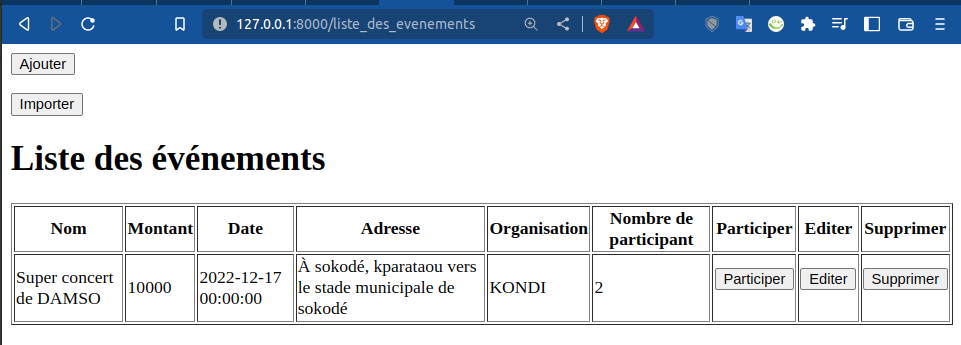
\includegraphics[scale=0.5]{img/fr.png}
\end{center}
EN :
\begin{center}
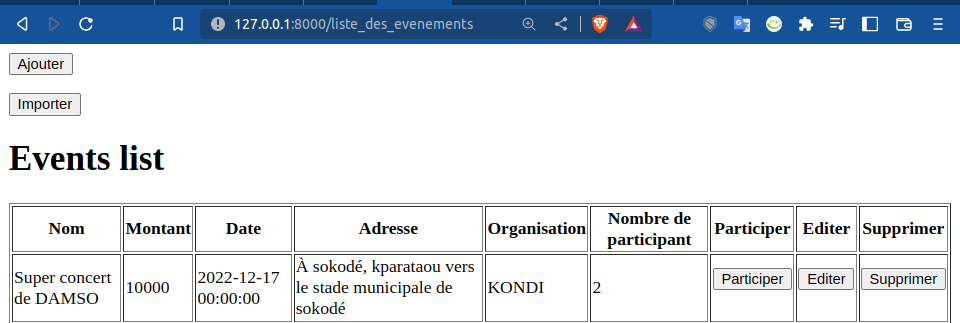
\includegraphics[scale=0.5]{img/en.png}
\end{center}

\subsection{DOM PDF}
Il existe plusieurs façon de générer un fichier pdf avec \textbf{PHP LARAVEL}. La méthode que 
nous allons voir ici est l'utilisation du Service \textbf{DOM PDF}.
Pour l'installer voici ce qu'il faut faire.

\begin{verbatim}
composer require barryvdh/laravel-dompdf
\end{verbatim}

Maintenant que le service est installer, essayons de générer un pdf lorsqu'on clique sur le bouton
participer. Pour le faire, nous allons modifier le fichier \textbf{evenement/index} comme ceci.
\begin{verbatim}
<td>{{ $event->organisateur }}</td>
<td></td>
<td>
	<form method="post" action="{{ route('generatePdf', $event) }}">
		@csrf
		<input type="submit" value="Participer">
	</form>
</td>
<td>
	<form method="get" action="{{route('formulaireEditerEvenement', $event)}}">
		@csrf
		<input type="submit" value="Editer">
	</form>
</td>
\end{verbatim}

Nous allons aussi créer la route \textbf{generatePdf} 
\begin{verbatim}
Route::post('genarate_pdf/{evenement}', [\App\Http\Controllers\EvenementController::class,
'genererPDF'])->name('generatePdf');
\end{verbatim}

Ensuite nous allons créer la méthode generatePDF dans le contrôleur EvenementController.
\begin{verbatim}
public function genererPDF(Evenement $evenement){

        //dd($evenement->organisateur());
        $pdf = Pdf::loadView('evenement.ticket', array(
            "evenement" => $evenement
        ));

        return $pdf->download('ticket.pdf');
}
\end{verbatim}
La méthode \textbf{genererPDF} nous permet de télécharger le pdf.

Enfin on créer une vue template \textbf{evenement/ticker.blade.php} comme ça.
\begin{verbatim}
<html>
<head>
    <meta charset="utf-8">
    <title>Liste</title>
</head>
<body>
    <main>
        <h1>Ticket de l'evenement : {{ $evenement->nom }}</h1>
        <fieldset>
            <div>
                <label>Nom : </label><label>{{ $evenement->nom }}</label>
            </div>
            <div>
                <label>Montant : </label><label>{{ $evenement->montant }}</label>
            </div>
            <div>
                <label>Date : </label><label>{{ \App\Helpers
                \EvenementHelper::afficherDateEtDate($evenement->date) }}</label>
            </div>
            <div>
                <label>Adresse : </label><label>{{ \App\Helpers
                \EvenementHelper::afficherAdresse($evenement->adresse) }}</label>
            </div>
            <div>
                <label>Organisateur : </label><label>{{-- $evenement->organisateur->nom." ".
                $evenement->organisateur->prenom --}}</label>
            </div>
        </fieldset>
    </main>
</body>
</html>
\end{verbatim}

Et voila le résultat.\\
\begin{center}
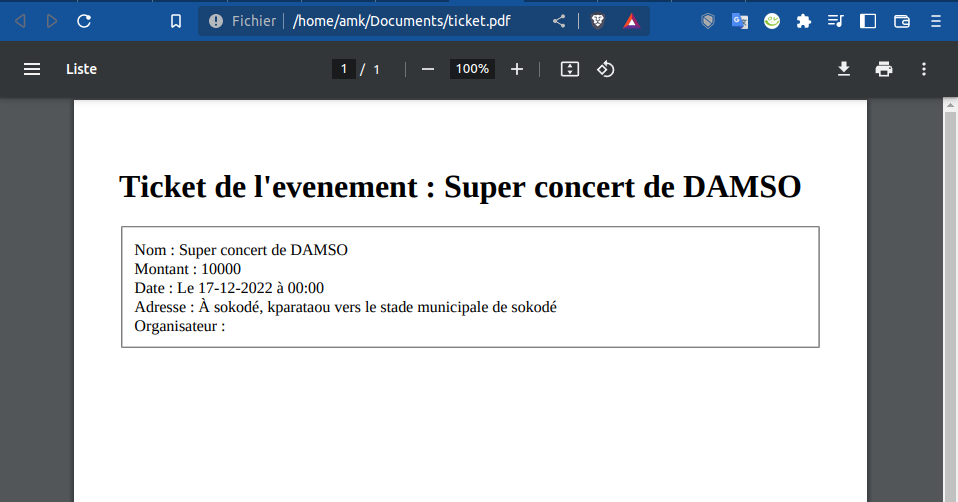
\includegraphics[scale=0.5]{img/pdf.png}
\end{center}


\subsection{Import et Export Excel}
Pour implémenter l'import en des données depuis un fichier Excel vers notre base de donné on utilise le
module . Voici comment on l'installe.

\begin{verbatim}
composer require maatwebsite/excel
php artisan vendor:publish --provider="Maatwebsite\Excel\ExcelServiceProvider" --tag=config
\end{verbatim}

\subsubsection{Import}
Si nous voulons importer une liste d'événements, on créer un modèle import correspondant a notre
notre modèle Evenement comme ceci.

\begin{verbatim}
php artisan make:import EvenementImport --model=Evenement
\end{verbatim}

Voici le contenue par défaut le la classe EvenementImport.
\begin{verbatim}
<?php

namespace App\Imports;

use App\Models\Evenement;
use Maatwebsite\Excel\Concerns\ToModel;

class EvenementImport implements ToModel
{
    /**
    * @param array $row
    *
    * @return \Illuminate\Database\Eloquent\Model|null
    */
    public function model(array $row)
    {
        return new Evenement([
            //
        ]);
    }
}
\end{verbatim}
Voici le format de notre fichier Excel.\\
\begin{center}
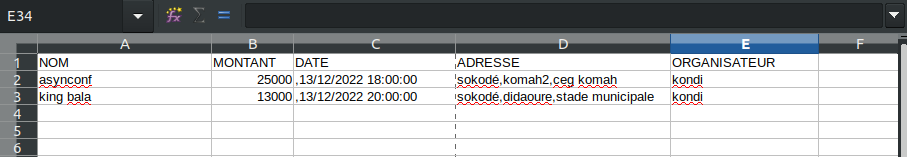
\includegraphics[scale=0.5]{img/fichier_excel.png}
\end{center}
Changer le contenue de la méthode model par ce qui suit.
\begin{verbatim}
<?php

namespace App\Imports;

use App\Models\Evenement;
use App\Models\User;
use Carbon\Carbon;
use Maatwebsite\Excel\Concerns\ToModel;

class EvenementImport implements ToModel
{
    /**
    * @param array $row
    *
    * @return \Illuminate\Database\Eloquent\Model|null
    */
    public function model(array $row)
    {
        if (! $row ?? "" && $row[0]==null){
            return null;
        }
        if ($row[0]=="NOM"){
            return null;
        }
        $adresse = explode(",", $row[3]);
        return new Evenement([
            'nom'=>strtoupper($row[0]),
            'montant'=>$row[1],
            'date'=>Carbon::createFromFormat("d/m/Y H:i:s", explode(",", $row[2])[1]),
            'adresse' => array(
                'ville' => $adresse[0],
                'quartier' => $adresse[1],
                'lieu' => $adresse[2],
            ),
            'organisateur' => User::all()->where('nom', strtoupper($row[4]))->first()->id_user,
        ]);
    }
}
\end{verbatim}

Maintenant que c'est fait, il nous faut créer deux routes une pour télécharger le fichier
excel et l'autre pour charger le contenue du fichier en base de donné comme ceci.
\begin{verbatim}
Route::get('formulaire_import_excel', [\App\Http\Controllers\EvenementController::class, 'importEvent'])->name('formulaireImportExcel');
Route::post('import_excel', [\App\Http\Controllers\EvenementController::class, 'importEventStore'])->name('importExcel');
\end{verbatim}

Évidement nous devons créer les deux méthode : importEvent et importEventStore.
Voici leur contenue.
\begin{verbatim}
public function importEvent()
    {
        return view('evenement.importExcel');
    }

public function importEventStore(Request $request)
    {
        $file = $request->file('fichierExcel'); // récupération le fichier
        $path = "fichier.".$file->extension(); // création d'un nom 
        $file->storeAs("public/", $path); // stockage du fichier
        Excel::import(new EvenementImport(), "public/".$path); // importer les données du fichier
        return redirect()->route('listeEvenements') //redirection;
    }
\end{verbatim}
\begin{itemize}
\item[•] La méthode \textbf{importEvent} est classique elle retourne le formulaire
d'import excel.
\item[•] La deuxième méthode \textbf{importEventStore} est quant à elle nous permet de stocker puis d’enregistrer les données du fichier excel dans la base. Mais pour que cela marche il faut créer un line symbolique vers le dossier storage avec la commande suivante.
\begin{verbatim}
php artisan storage:link
\end{verbatim}
Il nous faut aussi définir l'attribut \textbf{entype} de la balise form \textbf{multipart/form-data} en comme ceci.
\begin{verbatim}
<html>
<head>
    <meta charset="utf-8">
    <title>Liste</title>
</head>
<body>
<main>
    <h1>Formulaire d'enregistrement d'un événements.</h1>
    <form method="post" action="{{ route('importExcel') }}" enctype="multipart/form-data">
        @csrf
        <div>
            <input type="file" value="" name="fichierExcel">
        </div>
        <input type="submit" value="enregister">
    </form>
</main>
</body>
</html>
\end{verbatim}
\end{itemize}
Voici le résultat : \\
Avant l'import.
\begin{center}
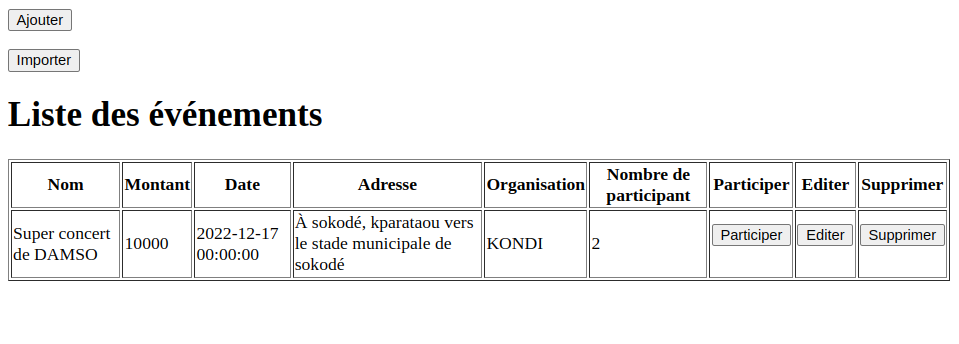
\includegraphics[scale=0.55]{img/before_import.png}
\end{center}
Choisissez votre fichier excel.
\begin{center}
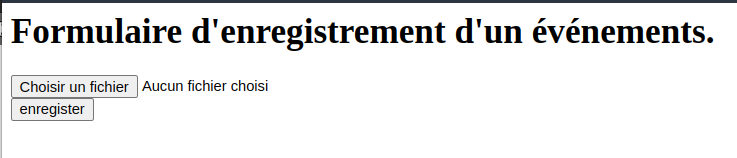
\includegraphics[scale=0.6]{img/import_form.png}
\end{center}
Après l'import.
\begin{center}
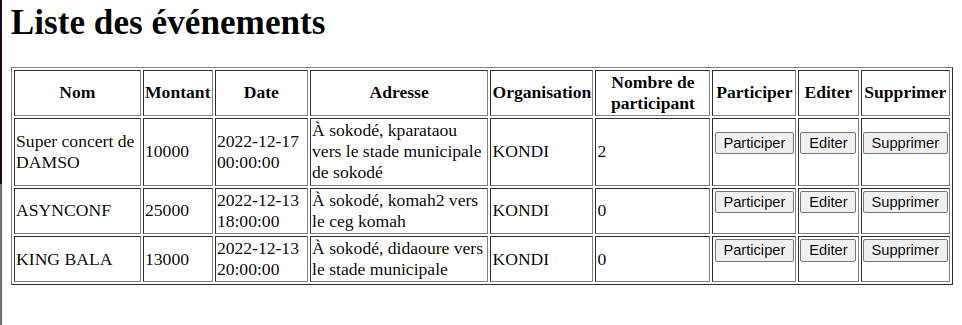
\includegraphics[scale=0.55]{img/import.png}
\end{center}

\subsubsection{Export}
Pour exporter notre la liste de nos événements dans un fichier excel. On procède comme
ceci : 
\begin{itemize}
\item[•] On créer une classe export comme ceci.
\begin{verbatim}
php artisan make:export EvenementExport --model=Evenement
\end{verbatim}
\item[•] Ensuite une route dans le fichier route/web.php.
\begin{verbatim}
Route::post('export_excel', [\App\Http\Controllers\EvenementController::class,
 'exportEvent'])->name('exportExcel');
\end{verbatim}
\item[•] Ensuit on crée la méthode \textbf{exportEvent}.
\begin{verbatim}
public function exportEvent(Request $request)
    {
        return Excel::download(new EvenementExport(), "liste_des_evenements.xlsx");
    }
\end{verbatim}
\item[•] Puis on créer un bouton de téléchargement dans la vue index.blade.php.
\begin{verbatim}
<form method="post" action="{{route('exportExcel')}}">
       @csrf
      <input type="submit" name="export" value="Exporter">
</form>
\end{verbatim}
\end{itemize}

Voici le résultat : \\
Avant l'export. \\
\begin{center}
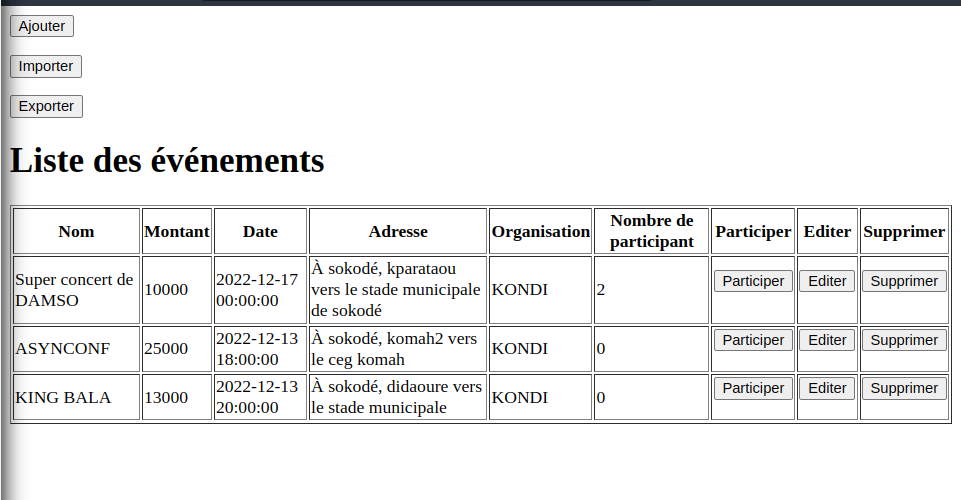
\includegraphics[scale=0.55]{img/export_index.png}
\end{center}
\begin{center}
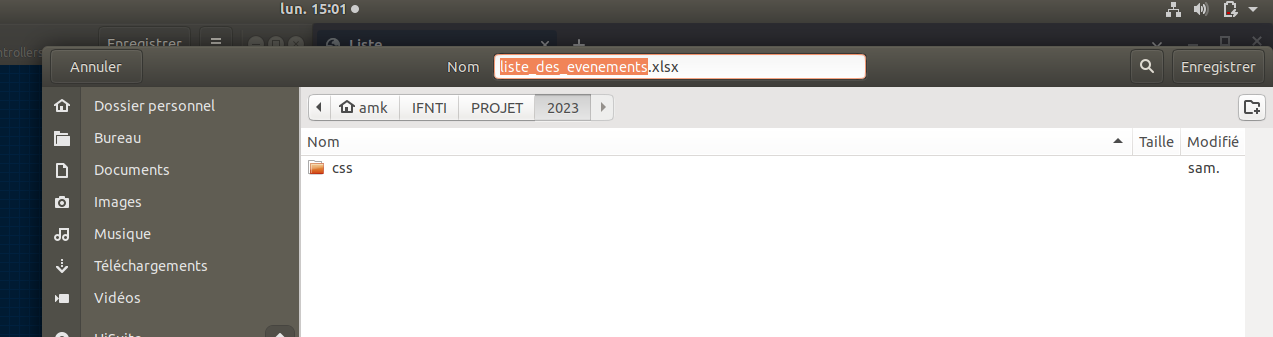
\includegraphics[scale=0.4]{img/export_d.png}
\end{center}
Après l'export. \\
\begin{center}
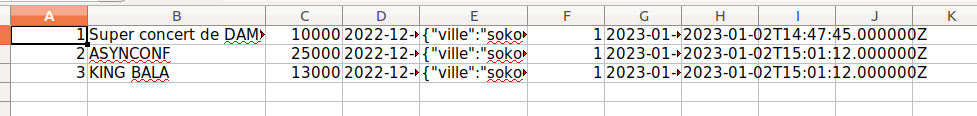
\includegraphics[scale=0.55]{img/export_file.png}
\end{center}

\section{Déploiements}
Il y-à plusieurs façons de déployer une application fait en Laravel sur un serveur d'application (Apache2, NginX). Ici nous allons voir comment utiliser \textbf{Apache2} pour
déployer notre site.\\
\textbf{NB:} Ceci est valide pour un déploiement sans logiciel de gestion de site web.\\

Avant de continuer créer un répertoire git pour votre projet. C'est fait ? alors on peut continuer...

\subsection{Sous linux}
Connecter vous à la machine sur le quelle vous devez faire et déploiement. Récupérer votre projet sur cette machine en faisant un \textit{git clone https://....} dans le répertoire 
\textbf{www}. Ensuit, 
installer vos dépendance : \textbf{php} et toute ses dépendance,\textbf{composer ...} et
\href{https://doc.ubuntu-fr.org/apache2}{apache 2}. Une fois apache installer sur votre 
système. Ouvrez un terminal et rendez vous au niveau de votre projet (cd ...). Pour le moment
démarrez le serveur de production, vous remarquerez que ça ne marche pas. \\
Quelle est l'erreur ? Comment compté vous la corriger ? Fait le.
Relancer le serveur. Ça ne marche toujours pas ! Quelle est l'erreur ? Comment compté vous la
corriger ? Fait le.
\textbf{NB:} Si vous avez des difficulté, sachez que les erreurs surgissent car le 
vendor et le .env n'existe plus (à cause de git).

Une fois que le vendor et le .env ont été recréer, relancer le serveur de production. Ça marche super. Arrêter le.

\textbf{NB :} Si vous avez d'autre type d'erreur comprenez les et essayé de le 
réglé. Le plus souvent ça peut être des module non installer (Ex: pdo) ou la base de 
donnée non configuré ou installé.

Changer le propriétaire de votre application en \textbf{www-data} comme ceci.
\begin{verbatim}
chown -R www-data:www-data nom_projet
\end{verbatim} 
Après rendez vous au niveau de votre du répertoire d'apache2.
\begin{verbatim}
cd /etc/apache2/
\end{verbatim} 
Puis créer un fichier de configuration pour votre application.
\begin{verbatim}
nano sites-available/mon_projet.conf
\end{verbatim}
Mettez s'y ceci.
\begin{verbatim}
<VirtualHost *:80>
    ServerAdmin admin@example.com
    ServerName name.com
    DocumentRoot projet_path/public

    <Directory projet_path>
    Options Indexes FollowSymlinks
    AllowOverride All
    Require all granted
    </Directory>

    SSLEngine on
    
    ErrorLog ${APACHE_LOG_DIR}/error.log
    CustomLog ${APACHE_LOG_DIR}/access.log combined
</VirtualHost>
\end{verbatim}
Sauvegardé et quitté. Monté maintenant le site  en faisant:
\begin{verbatim}
sudo a2dissite 000-default.conf 
sudo a2ensite mon_projet.conf
\end{verbatim}
Redémarrer votre serveur apache. Normalement si vous rendez au niveau de votre 
localhost vous pouvez remarquer que votre application à bien été hébergé.
\end{document}



